%from  intro
The urgency authority has received limited attention. \citet{siavelis.2002} is the only systematic study we are aware of. Analysis of Chile's first post-transition administration revealed the amazing frequency with which urgency messages were issued by President Aylwin: slightly more than one-third of proposals in Congress received some form of urgency, and about nine out of ten urgent bills were executive-initiated. Seeking whether or not urgent proposals had a more expedite legislative process and an improved likelihood of passage, the study found mixed evidence at best. Among executive proposals, urgent ones had somewhat shorter consideration than the rest (medians of 134 vs.\ 160 days, respectively). But no palpable difference in success rates could be appreciated (64 vs.\ 63 percent). 

The little power of the signal may bear relation to selection bias. Strategic presidents are likely to target for urgency proposals that differ from the rest in important ways, so the set of bills receiving urgent status is not random. Right censoring may also be an obstacle. A more fundamental problem is institutional indeterminacy. \citet{berrios.gamboa.fiscChile.2006} warn against overstating the Chilean urgency authority's importance, as non-compliance entails no penalty for Congress. %---unlike the Brazilian, Colombian, and Uruguayan variants.

Subsequent research, reviewed in section 2, showed that distinguishing types of urgency messages by degree---key for our argument---recovers some of the evidence that Siavelis missed. 

We offer an alternative interpretation of the urgency authority in Chile. The key is not how fast urgent proposals are considered, but the way they are considered in the floor. Restrictive rule. 


% from section
The urgency authority has received limited attention. \citet{siavelis.2002} is the only systematic study we are aware of. Analysis of Chile's first post-transition administration revealed the amazing frequency with which urgency messages were issued by President Aylwin: slightly more than one-third of proposals in Congress received some form of urgency, and about nine out of ten urgent bills were executive-initiated. He sought if urgent proposals had a more expedite legislative process and an improved likelihood of passage, finding mixed evidence at best. Among executive proposals, the urgent had somewhat shorter consideration than the rest (medians of 134 vs.\ 160 days, respectively). But no palpable difference in success rates could be appreciated (64 vs.\ 63 percent). 

The negative finding may bear relation to selection bias. Strategic presidents are likely to target for urgency proposals that are markedly different from the rest in important ways, so the set of bills receiving urgent status is not random. A more fundamental problem is that, unlike the Brazilian, Colombian, and Uruguayan variants, the consequences of congressional inaction on an urgent bill are indeterminate in Chile. \citet{berrios.gamboa.fiscChile.2006} warn against overstating the Chilean urgency authority's importance, as non-compliance entails no penalty for Congress. 

We offer an alternative interpretation of the urgency authority in Chile. importa porque es forma de restrictive rule. 



% from section






% from old section
The negative finding may bear relation to three elements. In their study of budgetary congressional oversight of the executive, \citet{berrios.gamboa.fiscChile.2006} warn against overstating the Chilean urgency authority's importance, as non-compliance entails no penalty for Congress---the next section develops this argument. While this may explain the lack of effects, it begs the question of why the president resorted so frequently to an authority that seems inconsequential. In other words, why make so many empty threats?


%% % longer review of aleman and navia
\citeauthor{aleman.navia.UrgChi.2009}'s \citeyearpar{aleman.navia.UrgChi.2009} systematic study of executive success in Congress in three post-transition presidencies also inspects Chile's urgency authority. Among controls, their equation includes urgency authority usage in the right side. The unit is the individual bill, and the size of the executive agenda varies substantially over the years. Variation is quantitative  (Congress received about 150 presidential bills in each of the first 6 years after 1990, a numbrer that dropped to about 70 in the next 6 years, then climbed to about 100 in the final 4 years of their series) and qualitative, presidents manifesting different propensities to aim at constitutional reform. Of direct relevance are the findings on urgencies. Controlling for key policy domains, chamber of origin, seat margins, and presidential approval, and clustering errors by legislative year, different prioritization reveal quite different effects in passage. `Act now' and `2-week' notices significantly increased the probability of bill passage, but not `one month' notices. 

Finally, selection bias is an obstacle to measure urgency authority effects. Presidents, behaving strategically, are likely to target for urgency proposals that are markedly different from the rest in important ways, so the set of bills receiveing urgent status is not random. Like the Siavelis and Alemán-Navia studies, we recognize the endogeneity problem that arises but does not confront it methodologically. Until a more subtle identification design is proposed, findings must be taken with a grain of salt. The systematic study of the urgency authority in Chile that follows should contribute to pave the way to a solution. 

%% %If presidents, behaving strategically, were to target for urgency proposals that are markedly different from the rest in important ways, a problem of endogeneity arises. Classify proposals based on how difficult passage is expected: easy, hard, and impossible. If left on their own, the easy proposals would be approved faster, the hard slower, the impossible never. A strategic president should concentrate the urgency authority in the hard group, leaving easy proposals mostly on their own, while abandoning the hopeless group of impossible proposals, that will not be observed. As a consequence, comparing

%% %The relevant quantity of interest is whether the use of the urgency authority affects bill passage (success, speed, amendments, and so forth) compared to the same bill with no urgency attached. The fundamental problem of causal inference is immediately evident. The executive presumably targets bills for urgency strategically, so that the selection mechanism cannot be assumed random. If, for example, more complex and divisive legislation takes longer, is likelier to fail and likelier to be tagged urgent, separating effects requires more subtle methods than used up to now.




% federalist 70
% Upon the principles of a free government, inconveniences from the source just mentioned [collective actors] must necessarily be submitted to in the formation of the legislature; but it is unneccessary, and therefore unwise, to introduce them into the constitution of the executive.
It is here too that they may be most pernicious.


When a resolution too is once taken, the opposition must be at an end. That resolution is a law, and resistance to it is punishable. --> EMM la urgencia opera contra esta delibaración benévola...

\section{El proceso de las indicaciones}

Para estilizar la secuencia de votación e indicación de un proyecto, consideramos un ejemplo simple. Se introduce un proyecto que contiene tres artículos. 

\begin{itemize}
\item Art 1. Se abre partida de \$200
\item Art 2. Se la divide por mitades
\item Art 3. Una mitad para alumnos, la otra para maestros
\end{itemize}

\noindent Si se aprobara, habría \$100 para maestros y alumnos. Si la mayoría quisiera entregarle \$150 a los maestros, podría hacer una indicación al art.\ 1, aumentando la partida a \$300. Problema: el único que puede hacerla en Chile es el ejecutivo. Si Hacienda se negase a gastar más, aún queda la ruta distributiva: menos para los alumnos, más para los maestros. Basta una enmienda al segundo artículo para dejar la distribución en $\frac{1}{3}$ y $\frac{2}{3}$. 

Notación:
\begin{itemize}
\item $p$ es el proyecto
\item $q$ es el status quo (todos reciben \$0)
\item $p_1$ es proyecto con art.\ 1 indicado
\item $p_2$ es proyecto con art.\ 2 indicado
\item $p_{12}$ es proyecto con arts.\ 1 y 2 indicados
\end{itemize}

La negociación procede así. Si la comisión de Hacienda admitiera la indicación al art.\ 1, el primer informe contaría con el proyecto $p$ y la versión modificada $p_1$. La discusión en general es un voto $p$ vs.\ $q$ primero. Si ganara $p$ (en algunos casos por supermayoría), seguiría un voto por la adminisilidad de la indicación, resultando $p1$ si ganara, $p$ si perdiera.

Regresa a comisión para un segundo informe. En él, se podría introducir la enmienda del art.\ 2, o $p_2$. La Figura \ref{f:agendaUrg} estiliza el proceso. Lo fundamental es que las urgencias sumas y de discusión inmediata (en Cámara, por lo menos) hacen que se prescinda del segundo informe y su duscusión. Así que urgencia = closed rule. [Hay que regresar a ley org. y reglamento para ver si la caricatura es acertada.]

Un perfil de preferencia para ilustrar podria ser:
\begin{itemize}
\item La mayoría está cerca de los maestros y ordena las alternativas $p_{12}>p_{2}>p_{1}>p>q$ (de mejor a peor)
\item El gobierno:  $p>q>p_2>p_1>p_{12}$.
\end{itemize}




\begin{sidewaysfigure}
  \centering
    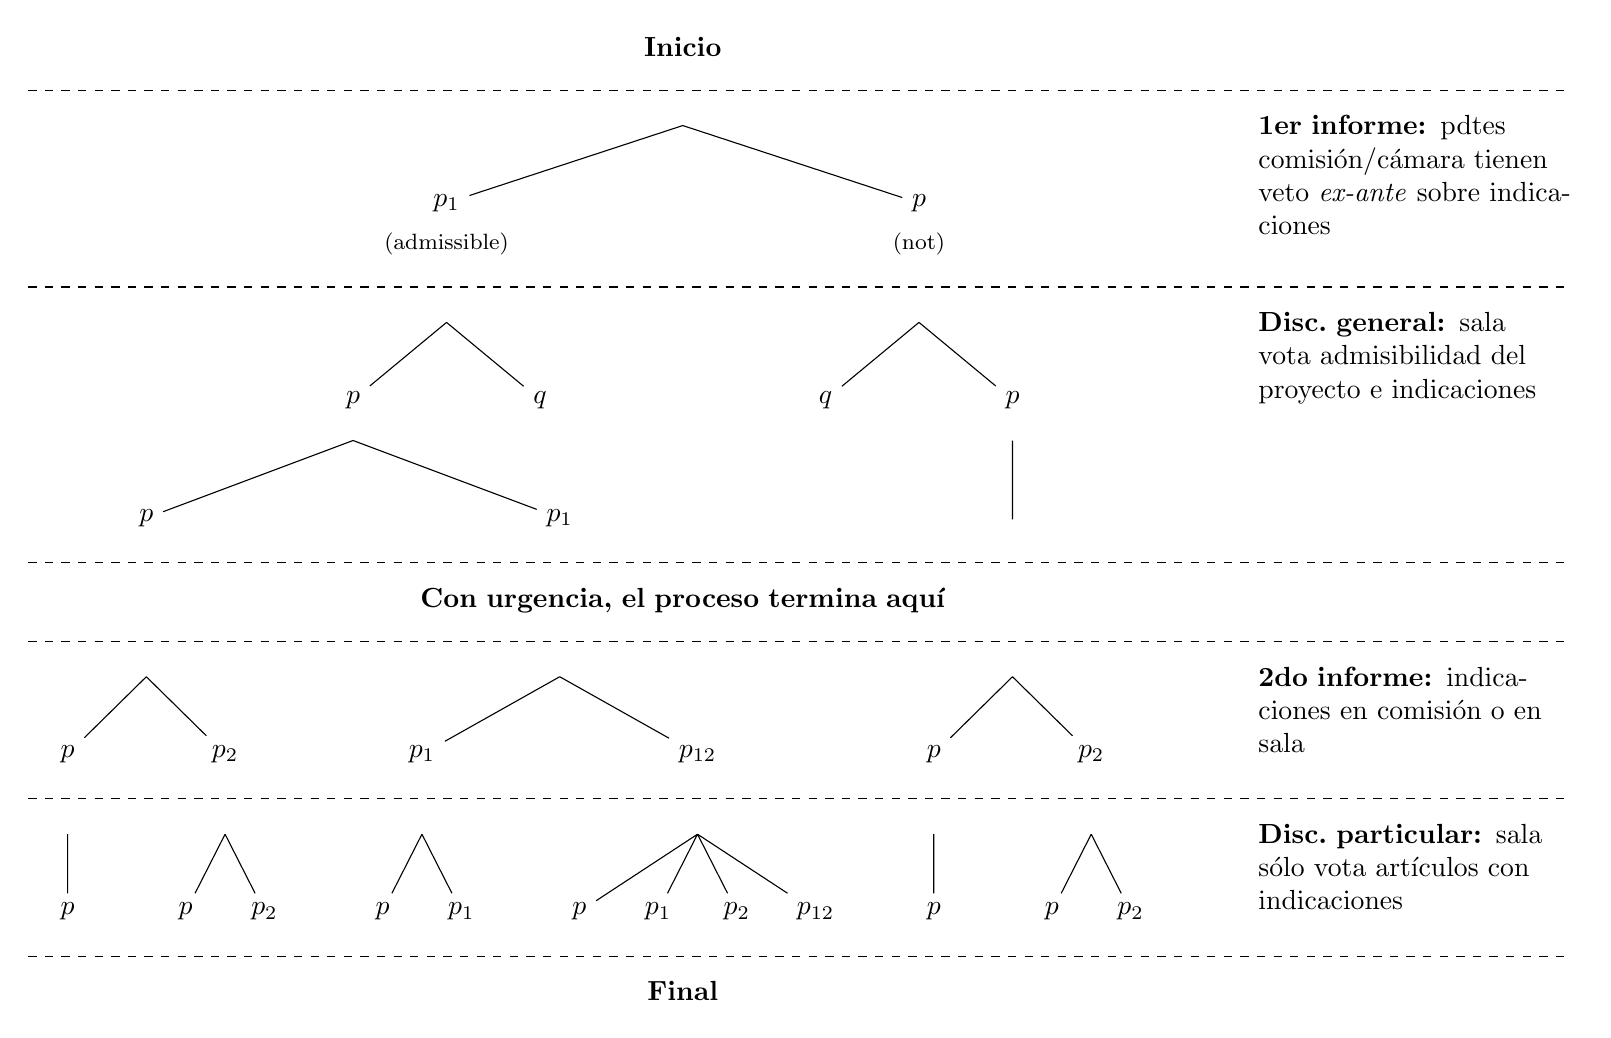
\begin{tikzpicture}
      \node[text width=10cm, text centered, anchor=north,fill=white] at (8.8125,-11) {\textbf{Final}}; 
      %%%%%%%%%%%%%%%%%%%%%%%%%%%%%%%%%%%%%%%%%%%%%%%
      \draw[dashed] (0.5,-10.8) -- (20,-10.8);
      %%%%%%%%%%%%%%%%%%%%%%%%%%%%%%%%%%%%%%%%%%%%%%%
      \node[below] at (1,-10)    (o1)  {$p$}; 
      \node[below] at (2.5,-10)  (o2)  {$p$}; 
      \node[below] at (3.5,-10)  (o3)  {$p_2$}; 
      \node[below] at (5,-10)    (o4)  {$p$}; 
      \node[below] at (6,-10)    (o5)  {$p_1$}; 
      \node[below] at (7.5,-10)  (o6)  {$p$}; 
      \node[below] at (8.5,-10)  (o7)  {$p_1$}; 
      \node[below] at (9.5,-10)  (o8)  {$p_2$}; 
      \node[below] at (10.5,-10) (o9)  {$p_{12}$}; 
      \node[below] at (12,-10)   (o10) {$p$}; 
      \node[below] at (13.5,-10) (o11) {$p$}; 
      \node[below] at (14.5,-10) (o12) {$p_2$}; 
      \draw (1,-9.25) -- (o1)
            (3,-9.25) -- (o2)
            (3,-9.25) -- (o3)
            (5.5,-9.25) -- (o4)
            (5.5,-9.25) -- (o5)
            (9,-9.25) -- (o6)
            (9,-9.25) -- (o7)
            (9,-9.25) -- (o8)
            (9,-9.25) -- (o9)
            (12,-9.25) -- (o10)
            (14,-9.25) -- (o11)
            (14,-9.25) -- (o12);
      \draw[dashed] (0.5,-8.8) -- (20,-8.8);
      \node[text width=4cm, anchor=north west,fill=white] at (16,-9) {\textbf{Disc.\ particular:} sala sólo vota artículos con indicaciones}; 
      %%%%%%%%%%%%%%%%%%%%%%%%%%%%%%%%%%%%%%%%%%%%%%%
      \node[below] at (1,-8) (i21) {$p$}; 
      \node[below] at (3,-8) (i22) {$p_2$}; 
      \node[below] at (5.5,-8) (i23) {$p_1$}; 
      \node[below] at (9,-8) (i24) {$p_{12}$}; 
      \node[below] at (12,-8) (i25) {$p$}; 
      \node[below] at (14,-8) (i26) {$p_2$}; 
      \draw (2,-7.25) -- (i21)
            (2,-7.25) -- (i22)
            (7.25,-7.25) -- (i23)
            (7.25,-7.25) -- (i24)
            (13,-7.25) -- (i25)
            (13,-7.25) -- (i26);
      \draw[dashed] (0.5,-6.8) -- (20,-6.8);
      \node[text width=4cm, anchor=north west,fill=white] at (16,-7) {\textbf{2do informe:} indicaciones en comisión o en sala}; 
      % %%%%%%%%%%%%%%%%%%%%%%%%%%%%%%%%%%%%%%%%%%%%%%%
      \draw[dashed] (0.5,-5.8) -- (20,-5.8);
      \node[text width=10cm, text centered, anchor=north,fill=white] at (8.8125,-6) {\textbf{Con urgencia, el proceso termina aquí}}; 
      %%%%%%%%%%%%%%%%%%%%%%%%%%%%%%%%%%%%%%%%%%%%%%%
      \node[below] at (2,-5) (g11) {$p$}; 
      \node[below] at (7.25,-5) (g12) {$p_1$}; 
      \node[below] at (4.625,-3.5) (g1) {$p$}; 
      \node[below] at (7,-3.5) (g2) {$q$}; 
      \node[below] at (13,-3.5) (g3) {$p$}; 
      \node[below] at (10.625,-3.5) (g4) {$q$}; 
      \draw (4.625,-4.25) -- (g11)
            (4.625,-4.25) -- (g12)
            (13,-4.25) -- (13,-5.25)
            (5.8125,-2.75) -- (g1)
            (5.8125,-2.75) -- (g2)
            (11.8125,-2.75) -- (g3)
            (11.8125,-2.75) -- (g4);
      \draw[dashed] (0.5,-2.3) -- (20,-2.3);
      \node[text width=4cm, anchor=north west,fill=white] at (16,-2.5) {\textbf{Disc.\ general:} sala vota admisibilidad del proyecto e indicaciones}; 
      %%%%%%%%%%%%%%%%%%%%%%%%%%%%%%%%%%%%%%%%%%%%%%%
      \node[below] at (5.8125,-1) (i11) {$p_1$}; 
      \node[text width=2cm, text centered] at (5.8125,-1.75) {\footnotesize{(admissible)}}; 
      \node[below] at (11.8125,-1) (i12) {$p$}; 
      \node[text width=2cm, text centered] at (11.8125,-1.75) {\footnotesize{(not)}}; 
      \draw (8.8125,-.25) -- (i11)
            (8.8125,-.25) -- (i12);
      \draw[dashed] (0.5,.2) -- (20,.2);
      \node[text width=4cm, anchor=north west,fill=white] at (16,0) {\textbf{1er informe:} pdtes comisión/cámara tienen veto \emph{ex-ante} sobre indicaciones}; 
      %%%%%%%%%%%%%%%%%%%%%%%%%%%%%%%%%%%%%%%%%%%%%%%
      \node[text width=10cm, text centered, anchor=north,fill=white] at (8.8125,1) {\textbf{Inicio}}; 
      %%%%%%%%%%%%%%%%%%%%%%%%%%%%%%%%%%%%%%%%%%%%%%%
    \end{tikzpicture}  \\
\caption{Stylization of the voting agenda. Notación: $p$ es un proyecto; $q$ el status quo; $p_1$, $p_2$ y $p_{12}$ son, respectivamente, enmiendas al primer artículo del proyecto, al segundo o a ambos. Vea el texto.}\label{f:agendaUrg}
\end{sidewaysfigure}


-----------------------------------


Committee chair is from
           pres  coal opp tot
  1998        9     7   1  17
  2002        6     7   4  17
  2006        3    15   0  18
  2010        5    11   6  22


  
\begin{table}
\begin{center}
\begin{tabular}{lrrrr}
\mc{5}{l}{\emph{~~Part A. Committee chairs, C\'amara de Diputados}} \\
Coalition             & 1998--2002 & 2002--06 & 2006--10 & 2010--14 \\ \hline
President's party     &  53        & 35       & 17       & 23       \\
Other coalition party &  41        & 41       & 83       & 50       \\
Opposition            &   6        & 24       & ---      & 27        \\ \hdashline
Total                 & 100        & 100      & 100      & 100      \\ 
N standing committees &  17        &  17      &  18      & 22      \\ \hline
\mc{5}{l}{\emph{~~Part B. Congressional seats}} \\
Coalition   & 1998--2002    & 2002--06 & 2006--10 & 2010--14 \\ \hline
\mc{5}{l}{\emph{~~Seats, C\'amara de Diputados}} \\
President's & 58            & 53       & 51       & 50       \\
Opposition  & 42            & 48       & 47       & 48       \\
Regional    &               &          & 3        & 2        \\ \hdashline
Total       & 100           & 100      & 100      & 100      \\ \hline
\mc{5}{l}{\emph{~~Seats, Senate}} \\
President's & 50            & 50       & 55       & 45       \\
Opposition  & 50            & 50       & 45       & 55       \\ \hdashline
Total       & $100^{\dagger}$ & 100      & 100      & 100      \\ \hline
\mc{5}{r}{\footnotesize{$^\dagger$vacant seats dropped}}
\end{tabular}
% \begin{tabular}{lrrrrrr}
% Coalition   & 1990--94 & 1994--98 & 1998--2002    & 2002--06 & 2006--10 & 2010--14 \\ \hline
% \mc{7}{l}{\emph{~~C\'amara de Diputados}} \\
% President's & 60       & 58       & 58            & 53       & 51       & 50       \\
% Opposition  & 40       & 42       & 42            & 48       & 47       & 48       \\
% Regional    &          &          &               &          & 3        & 2        \\ \hdashline
% Total       & 100      & 100      & 100           & 100      & 100      & 100      \\ \hline
% \mc{7}{l}{\emph{~~Senate}} \\
% President's & 48       & 46       & 50            & 50       & 55       & 45       \\
% Opposition  & 52       & 54       & 50            & 50       & 45       & 55       \\ \hdashline
% Total       & $100^*$  & $100^*$  & $100^{*\dagger}$ & 100      & 100      & 100      \\ \hline
% \mc{7}{l}{\footnotesize{Notes: $^*$ vacant seats dropped; $^\dagger$ margin varied above and below 50/50 due to vacancies.}}
% \end{tabular}
\caption{The president's status in Congress. Percent seats controlled by electoral lists in each chamber. The president's list in 1998--2010 was Concertaci\'on; it was Alianza afterwards. Regional list includes major-list splinters (from Christian Democrats and UDI). President's status in the Senate slightly and briefly oscilated above and below majority due to vacant seats. Source: prepared with information from \protect\url{www.camara.cl}.}\label{t:congressSeats}
\end{center}
\end{table}




%% \begin{table}
%% \begin{center}
%% \begin{tabular}{lrrrr}
%% List        & 1998--2002    & 2002--06 & 2006--10 & 2010--14 \\ \hline
%% \mc{5}{l}{\emph{~~C\'amara de Diputados}} \\
%% President's & 58            & 53       & 51       & 50       \\
%% Opposition  & 42            & 48       & 47       & 48       \\
%% Regional    &               &          & 3        & 2        \\ \hdashline
%% Total       & 100           & 100      & 100      & 100      \\ \hline
%% \mc{5}{l}{\emph{~~Senate}} \\
%% President's & 50            & 50       & 55       & 45       \\
%% Opposition  & 50            & 50       & 45       & 55       \\ \hdashline
%% Total       & $100^{\dagger}$ & 100      & 100      & 100      \\ \hline
%% \mc{5}{r}{\footnotesize{$^\dagger$vacant seats dropped}}
%% \end{tabular}
%% % \begin{tabular}{lrrrrrr}
%% % Coalition   & 1990--94 & 1994--98 & 1998--2002    & 2002--06 & 2006--10 & 2010--14 \\ \hline
%% % \mc{7}{l}{\emph{~~C\'amara de Diputados}} \\
%% % President's & 60       & 58       & 58            & 53       & 51       & 50       \\
%% % Opposition  & 40       & 42       & 42            & 48       & 47       & 48       \\
%% % Regional    &          &          &               &          & 3        & 2        \\ \hdashline
%% % Total       & 100      & 100      & 100           & 100      & 100      & 100      \\ \hline
%% % \mc{7}{l}{\emph{~~Senate}} \\
%% % President's & 48       & 46       & 50            & 50       & 55       & 45       \\
%% % Opposition  & 52       & 54       & 50            & 50       & 45       & 55       \\ \hdashline
%% % Total       & $100^*$  & $100^*$  & $100^{*\dagger}$ & 100      & 100      & 100      \\ \hline
%% % \mc{7}{l}{\footnotesize{Notes: $^*$ vacant seats dropped; $^\dagger$ margin varied above and below 50/50 due to vacancies.}}
%% % \end{tabular}
%% \caption{The president's status in Congress. Percent seats controlled by electoral lists in each chamber. The president's list in 1998--2010 was Concertaci\'on; it was Alianza afterwards. Regional list includes major-list splinters (from Christian Democrats and UDI). President's status in the Senate slightly and briefly oscilated above and below majority due to vacant seats. Source: prepared with information from \protect\url{www.camara.cl}.}\label{t:congressSeats}
%% \end{center}
%% \end{table}

%% The span offers variance in the size and status of the president's coalition in Congress. Given electoral list voting unity since the return to democracy \citep{carey.2002,aleman.saieg.coalUnityChile.2007}, the seats they control are a good indicator of the executive's legislative support. As Table \ref{t:congressSeats} reports, the president's coalition was always in control of the C\'amara, but has controlled Senate majorities between 2006 and 2010 only (coinciding with the first Bachelet administration). By requiring 67, 60, and 57 percent votes of each chamber, respectively, constitutional reform, constitution-interpreting legislation, and organic laws therefore always required votes across the aisle. 




% Table created by stargazer v.5.2 by Marek Hlavac, Harvard University. E-mail: hlavac at fas.harvard.edu
% Date and time: Tue, Jul 11, 2017 - 10:44:55 PM
% Requires LaTeX packages: dcolumn 
\begin{table}[!htbp] \centering 
  \caption{Regression results} 
  \label{} 
\begin{tabular}{@{\extracolsep{5pt}}lD{.}{.}{-3} D{.}{.}{-3} D{.}{.}{-3} D{.}{.}{-3} } 
\\[-1.8ex]\hline 
\hline \\[-1.8ex] 
 & \multicolumn{4}{c}{\textit{Dependent variable:}} \\ 
\cline{2-5} 
\\[-1.8ex] & \multicolumn{4}{c}{dv12} \\ 
\\[-1.8ex] & \multicolumn{3}{c}{\textit{logistic}} & \multicolumn{1}{c}{\textit{generalized linear}} \\ 
 & \multicolumn{3}{c}{\textit{}} & \multicolumn{1}{c}{\textit{mixed-effects}} \\ 
\\[-1.8ex] & \multicolumn{1}{c}{(1)} & \multicolumn{1}{c}{(2)} & \multicolumn{1}{c}{(3)} & \multicolumn{1}{c}{(4)}\\ 
\hline \\[-1.8ex] 
 Copartisan comm.~chair      &
                             &
 Multiple referrals          &
                             &
 Member bill                 &
                             &
 Member bill, opp.-sponsored &
                             &
 Member bill, mix.-sponsored &
                             &
 Member bill, pres. coal.-sp.&
                             &
 Hacienda referral           &
                             &
 Year remaining              &
                             &
 Pres.~approval              &
                             &
 Introduced Senate           &
                             &
 Senate majority             &
                             &
 Relax deadlines             &
                             &
 2002-06 Leg.                &
                             &
 2006-10 Leg.                &
                             &
 2010-14 Leg.                &
                             &
 Constant                    &
                             &
\hline \\[-1.8ex] 
Observations & \multicolumn{1}{c}{6,987} & \multicolumn{1}{c}{6,987} & \multicolumn{1}{c}{6,987} & \multicolumn{1}{c}{6,987} \\ 
Log Likelihood & \multicolumn{1}{c}{-1,718} & \multicolumn{1}{c}{-1,702} & \multicolumn{1}{c}{-1,688} & \multicolumn{1}{c}{-1,695} \\ 
Akaike Inf. Crit. & \multicolumn{1}{c}{3,456.650} & \multicolumn{1}{c}{3,428.021} & \multicolumn{1}{c}{3,402.008} & \multicolumn{1}{c}{3,415.824} \\ 
Bayesian Inf. Crit. &  &  &  & \multicolumn{1}{c}{3,504.898} \\ 
\hline 
\hline \\[-1.8ex] 
\textit{Note:}  & \multicolumn{4}{r}{$^{*}$p$<$0.1; $^{**}$p$<$0.05; $^{***}$p$<$0.01} \\ 
\end{tabular} 
\end{table} 
> 


Including the Finance committee in the `other committee' count increases multiple referrals to 32 percent of bills.

 
